% Genuine tau_h decays compared with the objects that HPS can reconstruct in the same decay mode,
% for Chapter III (fig:tau_fakes). Same style as the tau decay modes of Chapter II (fig:tau_DMs).
% Adapted from https://tikz.net/tau_decay/ (Izaak Neutelings, CC BY-SA 4.0).
\documentclass[11pt,border=2pt]{standalone}
\usepackage[T1]{fontenc}
\usepackage{cochineal}
\usepackage[cochineal]{newtxmath}
\usepackage{tikz}
\usetikzlibrary{decorations.markings,decorations.pathmorphing}
\tikzset{>=latex}

% vertical custom shading (for the shower cones)
% https://tex.stackexchange.com/questions/191735
\makeatletter
\tikzset{vertical custom shading/.code={%
  \pgfmathsetmacro\tikz@vcs@middle{#1}
  \pgfmathsetmacro\tikz@vcs@bottom{\tikz@vcs@middle/2}
  \pgfmathsetmacro\tikz@vcs@top{(100-\tikz@vcs@middle)/2+\tikz@vcs@middle}
  \pgfdeclareverticalshading[tikz@axis@top,tikz@axis@middle,tikz@axis@bottom]{newaxis}{100bp}{%
    color(0bp)=(tikz@axis@bottom);
    color(\tikz@vcs@bottom bp)=(tikz@axis@bottom);
    color(\tikz@vcs@middle bp)=(tikz@axis@middle);
    color(\tikz@vcs@top bp)=(tikz@axis@top);
    color(100bp)=(tikz@axis@top)}
    \pgfkeysalso{/tikz/shading=newaxis}
  }
}
\makeatother
\tikzset{
  ->-/.style={decoration={markings,mark=at position .7 with {\arrow{>}}},postaction={decorate}},
  photon/.style={decorate,decoration={snake,segment length=5,amplitude=1.1}},
  mycone/.pic={
    \shadedraw[top color=white,bottom color=black!50,shading angle=50,vertical custom shading=10]
      (-0.4,0.99) -- (0,0) -- (0.4,0.99);
    \shadedraw[top color=white,bottom color=black!20,shading angle=90]
      (0,1) ellipse (0.4 and 0.12);}
}

\begin{document}
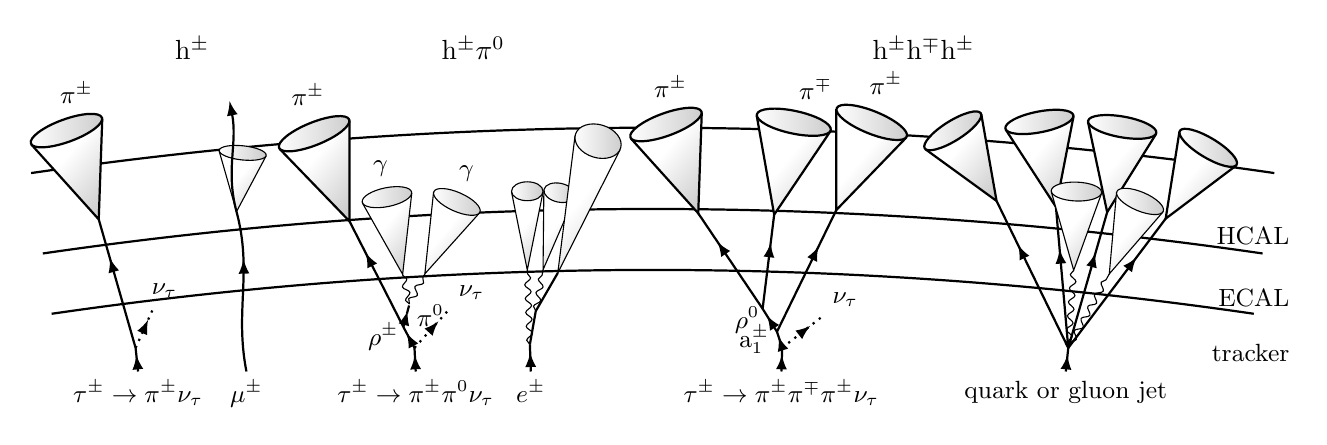
\begin{tikzpicture}[scale=0.43,every node/.style={font=\small}]
  \def\R{120}     % inner radius of the arcs
  \def\hca{8.3}   % half central angle
  \def\tracker{3}
  \def\ECAL{4.8}
  \def\HCAL{7.2}
  \pgfmathsetmacro\hclmax{(\R+\HCAL)*sin(\hca)}

  % detector layers
  \foreach \r in {\tracker,\ECAL,\HCAL}{
    \draw[thick] (0,\r) arc (90:90-\hca:\R+\r) (0,\r) arc (90:90+\hca:\R+\r);
  }
  % layer names at the right end, following the curvature of the arcs
  \node[above left] at ({1.04*\hclmax},0.0) {tracker};
  \node[above left] at ({1.04*\hclmax},1.62) {ECAL};
  \node[above left] at ({1.04*\hclmax},3.45) {HCAL};

  % decay mode reproduced by each pair, above the detector
  \foreach \x/\dm in {-13.6/{h$^\pm$},-5.3/{h$^\pm\pi^0$},8.0/{h$^\pm$h$^\mp$h$^\pm$}}
    \node[font=\normalsize] at (\x,9.55) {\dm};

  % ---------------- PAIR 1: one prong vs muon ----------------
  % genuine tau -> pi nu
  \begin{scope}[shift={(-15.2,0)},rotate=6]
    \node[below] at (0,0) {$\tau^\pm\to\pi^\pm\nu_\tau$};
    \draw[->-,thick] (0,0) -- (0,0.7) coordinate (tau);
    \draw[->-,dotted,thick,rotate=-30] (tau) --+ (0,1.3) node[right=4pt,above] {$\nu_\tau$};
    \draw[->-,thick,rotate=10] (tau) --+ (0,3.95) node[left=8,above=38] {$\pi^\pm$}
      pic[rotate=20,scale=1.2] {mycone};
  \end{scope}
  % muon crossing the calorimeters
  \begin{scope}[shift={(-12.0,0)},rotate=5]
    \node[below] at (0,0) {$\mu^\pm$};
    \draw[->-,thick] (0,0) to[out=96,in=-80] (0.12,4.73) coordinate (mu);
    \path (mu) pic[rotate=-6,scale=0.75] {mycone};
    \draw[->,thick] (mu) to[out=100,in=-84] (0.2,8.0);
  \end{scope}

  % ---------------- PAIR 2: one prong plus strip vs electron ----------------
  % genuine tau -> rho nu -> pi pi0 nu
  \begin{scope}[shift={(-7.0,0)},rotate=3]
    \node[below] at (0,0) {$\tau^\pm\to\pi^\pm\pi^0\nu_\tau$};
    \draw[->-,thick] (0,0) -- (0,0.7) coordinate (tau);
    \draw[->-,dotted,thick] (tau) --+ (45:1.5) node[above right] {$\nu_\tau$};
    \draw[->-,thick] (tau) --+ (115:0.7) coordinate (rho) node[midway,left] {$\rho^\pm$};
    \draw[->-,thick] (rho) --+ (114:3.5) node[left=15,above=38] {$\pi^\pm$}
      pic[rotate=22,scale=1.2] {mycone};
    \draw[->-,densely dashed,thick] (rho) --+ (72:0.7) coordinate (pion0) node[midway,right] {$\pi^0$};
    \draw[photon] (pion0) --+ (100:0.9) node[left=8,above=32] {$\gamma$}
      pic[rotate=11.5,xscale=0.8] {mycone};
    \draw[photon] (pion0) --+ (60:1.0) node[right=15,above=30] {$\gamma$}
      pic[rotate=-24,xscale=0.8] {mycone};
  \end{scope}
  % electron radiating bremsstrahlung photons, showering in the ECAL and leaking into the HCAL
  \begin{scope}[shift={(-3.6,0)},rotate=2]
    \node[below] at (0,0) {$e^\pm$};
    \draw[->-,thick] (0,0) -- (0,0.8) coordinate (b1);
    \draw[thick] (b1) -- ++(78:1.0) coordinate (b2);
    \draw[thick] (b2) -- ++(58:1.3) coordinate (e);
    \draw[photon] (b1) -- ++(90:2.2)
      pic[rotate=0,xscale=0.5] {mycone};
    \draw[photon] (b2) -- ++(78:1.24)
      pic[rotate=-12,xscale=0.5] {mycone};
    \path (e) pic[rotate=-17,xscale=0.75,yscale=1.75] {mycone};
  \end{scope}

  % ---------------- PAIR 3: three prongs vs quark or gluon jet ----------------
  % genuine tau -> a1 nu -> 3 pi nu
  \begin{scope}[shift={(3.8,0)},rotate=-2]
    \node[below] at (0,0) {$\tau^\pm\to\pi^\pm\pi^\mp\pi^\pm\nu_\tau$};
    \draw[->-,thick] (0,0) -- (0,0.7) coordinate (tau);
    \draw[->-,dotted,thick] (tau) --+ (40:1.5) node[above right] {$\nu_\tau$};
    \draw[->-,thick] (tau) --+ (110:0.5) coordinate (a1) node[midway,left] {a$_1^\pm$};
    \draw[->-,thick] (a1) --+ (124:0.8) coordinate (rho) node[midway,left] {$\rho^0$};
    \draw[->-,thick] (rho) --+ (126:3.4) node[left=10,above=38] {$\pi^\pm$}
      pic[rotate=20,scale=1.2] {mycone};
    \draw[->-,thick] (rho) --+ (85:2.8) node[right=15,above=38] {$\pi^\mp$}
      pic[rotate=-12,scale=1.2] {mycone};
    \draw[->-,thick] (a1) --+ (66:4.0) node[right=18,above=38] {$\pi^\pm$}
      pic[rotate=-22,scale=1.2] {mycone};
  \end{scope}
  % quark or gluon jet: more particles, spread over a wider angle
  \begin{scope}[shift={(12.2,0)},rotate=-6]
    \node[below] at (0,0) {quark or gluon jet};
    \draw[->-,thick] (0,0) -- (0,0.7) coordinate (q);
    \draw[->-,thick] (q) --+ (122:4.83) pic[rotate=32,scale=1.05] {mycone};
    \draw[->-,thick] (q) --+ (101:4.18) pic[rotate=11,scale=1.1] {mycone};
    \draw[->-,thick] (q) --+ (80:4.17)  pic[rotate=-10,scale=1.1] {mycone};
    \draw[->-,thick] (q) --+ (59:4.78)  pic[rotate=-31,scale=1.05] {mycone};
    \draw[photon] (q) --+ (92:2.3)  pic[rotate=-2,xscale=0.8] {mycone};
    \draw[photon] (q) --+ (67:2.5)  pic[rotate=-23,xscale=0.8] {mycone};
  \end{scope}
\end{tikzpicture}
\end{document}
